\section{Conmutación Segmentada}\label{sec:p01intro}\pagenumbering{arabic}

\subsection{Objetivo}\label{ssec:p01objetivo}

\normalsize Asimilar el funcionamiento de wormhole y comprender la utilidad de incluir canales virtuales
en el diseño de las redes de interconexión.


\subsection{Desarrollo}\label{ssec:p01desarrollo}

La práctica consiste en resolver una serie de cuestiones relacionadas con la técnica de
conmutación wormhole. Para realizar esta práctica se hará uso del simulador SimuRed, descrito en
el apéndice A. Debéis poner a cero los paquetes iniciales de precalentamiento o de relleno, para que
obtenga adecuadamente las estadísticas.

\begin{itemize}
    \item[\textbf{a)}] \textbf{Para comprobar la manera en la que se produce la transmisión de datos cuando se aplica wormhole, selecciona una topología toro 2D 4 × 4, con buffers con capacidad para 2 flits, paquetes de 3 flits (incluida la cabecera), retardos de 1 ciclo, encaminamiento determinista y un canal virtual; y simula la transferencia de 2 paquetes: uno enviado desde el nodo 0 al nodo 5 y otro enviado desde el nodo 2 también al nodo 5. Ambos envíos comienzan en el ciclo 0.}

    La única complejidad en este apartado es la de hacer una traza que recoja los paquetes que nos piden. Para ello, será necesario crear un fichero de texto con la extensión \verb|.trc| y en el incluir una línea por cada paquete que se quiera enviar (en el manual del simulador se explican con más detalle los campos que incluir en cada línea). El Listing \ref{lst:traza} muestra el resultado.

    \begin{mycode}[style=mycodestyle, caption={Traza a simular.}, label=lst:traza]
0 0 5
0 2 5
    \end{mycode}

    Durante la ejecución de la traza paso a paso, es interesante ver lo que ocurre cuando ambos paquetes compiten por los recursos en el nodo 1. En este caso, ante la colisión, el paquete proveniente del nodo 0 pasa primero, flit a flit. Además, cuando dicho paquete termina de salir de este nodo, el segundo paquete le sigue inmediatamente, pudiéndose apreciar la principal diferencia con \textit{Virtual Cut-Through}, ya que con esta técnica de conmutación, el paquete entero se bloquearía en el buffer del nodo 1 hasta que los buffers de entrada del nodo 5 estuviesen completamente libres, ya que la conmutación se realiza a nivel de paquete.

    \begin{keyconceptbox}[Wormhole]
        Es una técnica de conmutación en la que el control de flujo se ejerce sobre cada uno de los flits en los que se divide el mensaje, al contrario que en el \textit{Virtual Cut-Through}, en la que el control de flujo se lleva a cabo a nivel de paquete. Esto significa que el tamaño de los buffers se reduce mucho en wormhole, ya que sólo se tienen que asegurar los recursos para un flit, no para el paquete entero. La latencia viene dada por la siguiente fórmula:

        \begin{equation*}
        T_{WH} = D(t_r + t_s + t_w) + max(t_s,t_c)\left\lceil\frac{L}{W}\right\rceil
        \end{equation*}
        
    \end{keyconceptbox}

    \begin{keyconceptbox}[Toro]
        Es un tipo de topología de red directa y ortogonal. Pertenece a la familia de topologías $n$-cubo $k$-arias. En un toro, cada nodo está conectado con dos vecinos a lo largo de dos o más dimensiones. Un toro 2D 4x4 se podría visualizar como cuatro colgantes de perlas cerrados, con cuatro perlas cada uno. Estos cuatro colgantes estarían dispuestos verticalmente, de manera que cada perla estuviera en línea y conectada con la inmediatamente superior y la inferior. Además, cada perla de la cadena más superior, estaría conectada a la perla correspondiente de la cadena más inferior. Estas características, diferencian al toro de la malla, ya que los nodos situados en los extremos de esta, no están conectados entre sí.

        \vspace{10pt}

        \centering 	\fbox{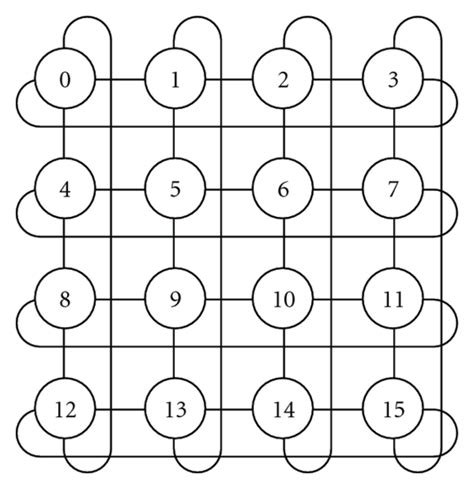
\includegraphics[width=0.5\linewidth]{figs/red-toroidal.jpeg}} \label{fig:red-toroidal}
    \end{keyconceptbox}

    \item[\textbf{b)}] \textbf{Para el ejemplo del apartado anterior, analiza los resultados estadísticos que se obtienen, explicando cada uno de ellos. Repite la misma simulación para otros tamaños de paquete y de buffer (8 y 32 flits, por ejemplo). Observa lo que ocurre y comenta los resultados (indica lo que ocurre cuando los paquetes deben usar el mismo canal o lo que pasa cuando el tamaño del paquete es mucho mayor que el del buffer).}

    Tras salir del cuadro de simulación interactiva, en el recuadro blanco de la pestaña de simulación se muestran las estadísticas de la simulación. A continuación se muestran los resultados obtenidos tras simular la traza del apartado anterior. Dentro de dichas estadísticas se incluyen diferentes tasas:

    \begin{itemize}
        \item Tasa de creación = nº total de flits / nº total de ciclos / nº total de nodos
        \item Tasa de envíos = nº total de flits / nº total de nodos
        \item Tasa de recepción = nº total de flits / nº total de ciclos / nº total de nodos
    \end{itemize}
    
    \begin{mycode}[style=mycodestyle]
--------------------------------------------
Item: 1, Variable: 0.3
--------------------------------------------
Ciclos: 14
Paquetes Generados: 2
Paquetes Enviados:  2
Paquetes Recibidos: 2
---------------------------------------
Tasa  Creacion (flits/ciclo/nodo): 0.0267857142857143
Tasa de  Envio (flits/ciclo/nodo): 0.375
Tasa Recepcion (flits/ciclo/nodo): 0.0267857142857143
---------------------------------------
Latencia Cabeza:                 10
Latencia Cabeza (sin bloqueos):  8
Latencia Paquete:                12
Desviacion Estandar:             2
Latencia Paquete (sin bloqueos): 10
Ciclos de Bloqueo en Red:        2
--------------------------------
Camino medio (nodos):        3
Camino medio (canales):      2
 

SIMULACION COMPLETADA CON EXITO.
Tiempo de simulacion: 0 h, 0 m, 3 s.
    \end{mycode}

    \textit{¿Qué ocurre cuando los paquetes deben usar el mismo canal?} Lo que ocurre es que se produce una situación de bloqueo, ya que para salir del nodo 1, solo existe un buffer de salida. Al llegar al mismo tiempo ambos paquetes, uno de ellos se tiene que bloquear para que el otro paquete use el buffer.
    
    \textit{¿Qué pasa cuando el tamaño del paquete es mucho mayor que el del buffer?} Lo que ocurre es que el paquete que usa primero el buffer, lo retiene durante más ciclos, aumentando a su vez los ciclos de bloqueo y, en definitiva, la latencia media de la comunicación.
 

    \item[\textbf{c)}] \textbf{¿Cuál es la diferencia de funcionamiento si está activado o no el adelantamiento en colas o buffers?}

    La diferencia es que cuando el adelantamiento en colas está activado, el flit que entre en una cola se colocará en la primera posición libre de esta, mientras que con el adelantamiento desactivado dicho flit se colocaría al final de la cola y tendría que atravesar todas las posiciones intermedias para llegar al comienzo de la cola. La consecuencia del adelantamiento de colas es que se reduce la latencia, pues se reducen el número de ``saltos'' que el paquete tiene que dar hasta llegar a su destino. Esta diferencia será más evidente cuanto mayor sea el tamaño del buffer.

    \item[\textbf{d)}] \textbf{Propón como deberías configurar el simulador para que funcionara como VCT. }
    
    VCT realiza la conmutación a nivel de paquete, por lo que un nodo no puede aceptar un paquete si no puede asegurar que, en caso de bloqueo, puede almacenar el mensaje entero. Por lo tanto, para simular VCT en el simulador, bastaría con incrementar el tamaño de las colas por encima del tamaño de los paquetes.

    \item[\textbf{e)}] \textbf{Reproduce una situación en la que se muestre cómo el uso de canales virtuales puede reducir la contención provocada por wormhole, y con ello aumentar la utilización de los canales.}
    
    Simplemente con aumentar el número de canales virtuales a dos, se aprecia la diferencia, en especial si el tamaño de los paquetes es muy grande. En este caso, el paso de los paquetes de un nodo a otro se lleva a cabo de manera multiplexada en el tiempo, ya que el cable que los une es compartido por ambos paquetes, a pesar de que los exista un buffer para cada paquete. De esta manera, cuando ambos paquetes llegan al buffer de salida, el envío a través del cable que conecta ambos nodos se realiza de manera alterna: en $t_i$ pasa pasa un flit de un paquete, y en $t_{i+1}$ pasa un flit del otro paquete. 

    Si en el simulador aumentamos el tamaño de los buffers y desactivamos el adelanto en colas, se aprecia mejor la alternancia (véase la Figura \ref{fig:canales-virtuales}).

    \begin{figure}[h] % Adjust the width as needed
      \centering
      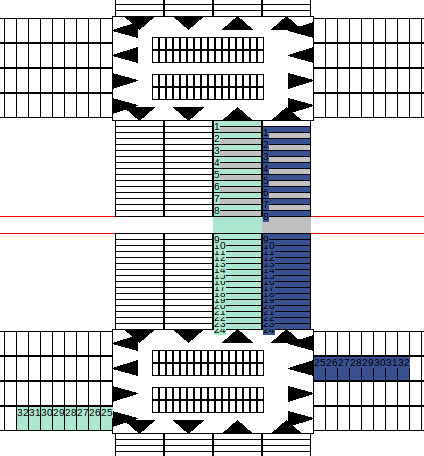
\includegraphics[width=0.3\textwidth]{figs/canales-virtuales.png} % Replace with your image filename
      \caption{Canales virtuales.}
      \label{fig:canales-virtuales}
    \end{figure}

\end{itemize}